%compile with pdflatex on papeeria

\documentclass[a4paper,12pt]{article}
\usepackage{fancyhdr}
\usepackage{fancyheadings}
\usepackage[ngerman,german]{babel}
\usepackage{german}
\usepackage[utf8]{inputenc}
%\usepackage[latin1]{inputenc}
\usepackage[active]{srcltx}
%\usepackage{algorithm}
%\usepackage[noend]{algorithmic}
\usepackage{amsmath}
\usepackage{amssymb}
\usepackage{amsthm}
\usepackage{bbm}
\usepackage{enumerate}
\usepackage{graphicx}
\usepackage{ifthen}
\usepackage{listings}
\usepackage{enumitem}
%\usepackage{struktex}
\usepackage{hyperref}
\usepackage{tikz}
\usepackage{float}
\usepackage{subcaption}
\captionsetup{compatibility=false}
\captionsetup[subfigure]{labelformat=empty}

\usepackage{pgfplots}
\usepgfplotslibrary{fillbetween}
%\usetikzlibrary{patterns}
\pgfplotsset{compat=1.15}
\usepackage{mathrsfs}
\usetikzlibrary{arrows}

\pgfplotsset{grid style={dashed,gray}}

\definecolor{ccqqqq}{rgb}{0.8,0,0}

\pagenumbering{gobble}

%%%%%%%%%%%%%%%%%%%%%%%%%%%%%%%%%%%%%%%%%%%%%%%%%%%%%%
%%%%%%%%%%%%%% EDIT THIS PART %%%%%%%%%%%%%%%%%%%%%%%%
%%%%%%%%%%%%%%%%%%%%%%%%%%%%%%%%%%%%%%%%%%%%%%%%%%%%%%
\newcommand{\Fach}{2. Klausur aus der Mathematik (A)}
\newcommand{\Name}{}
\newcommand{\datum}{}
\newcommand{\Matrikelnummer}{}
\newcommand{\Semester}{Q12/1}
\newcommand{\Uebungsblatt}{} %  <-- UPDATE ME
%%%%%%%%%%%%%%%%%%%%%%%%%%%%%%%%%%%%%%%%%%%%%%%%%%%%%%
%%%%%%%%%%%%%%%%%%%%%%%%%%%%%%%%%%%%%%%%%%%%%%%%%%%%%%

\setlength{\parindent}{0em}
\topmargin -1.0cm
\oddsidemargin 0cm
\evensidemargin 0cm
\setlength{\textheight}{9.2in}
\setlength{\textwidth}{6.0in}

%%%%%%%%%%%%%%%
%% Aufgaben-COMMAND
\newcommand{\Aufgabe}[1]{
  {
  \vspace*{0.5cm}
  \textsf{\textbf{Aufgabe #1}}
  \vspace*{0.2cm}
  
  }
}
%%%%%%%%%%%%%%
\hypersetup{
    pdftitle={\Fach{}: Übungsblatt \Uebungsblatt{}},
    pdfauthor={\Name},
    pdfborder={0 0 0}
}

\lstset{ %
language=java,
basicstyle=\footnotesize\tt,
showtabs=false,
tabsize=2,
captionpos=b,
breaklines=true,
extendedchars=true,
showstringspaces=false,
flexiblecolumns=true,
}

\title{Übungsblatt \Uebungsblatt{}}
\author{\Name{}}

\begin{document}
\thispagestyle{fancy}
%\lhead{\sf \large \Fach{} \\ %\small \Name{} - \Matrikelnummer{}
\lhead{\sf \large \Fach{} %\small \Name{} - \Matrikelnummer{}
}
\rhead{\sf \Semester{}   \datum{}}
%\rhead{\sf \Semester{} }
\vspace*{0.2cm}
%\begin{center}
%%\LARGE \sf \textbf{Übungsblatt \Uebungsblatt{}}
%\end{center}
%\vspace*{0.2cm}

%%%%%%%%%%%%%%%%%%%%%%%%%%%%%%%%%%%%%%%%%%%%%%%%%%%%%%
%% Insert your solutions here %%%%%%%%%%%%%%%%%%%%%%%%
%%%%%%%%%%%%%%%%%%%%%%%%%%%%%%%%%%%%%%%%%%%%%%%%%%%%%%

  Name: \underline{\hspace{7cm}}
%\draw[line width=1pt,color=ccqqqq,smooth,samples=100,domain=-6:7] plot(\x,{(1/12)*\x*\x+(1/3)*\x});
  \hfill
  Datum: \underline{\hspace{4cm}}

%\vspace{0,5cm}Die Rechenwege müssen nachvollziehbar sein!

\vspace{0,5cm} {TEIL A} - ohne Hilfsmittel
\vspace {0,2cm}
 

\Aufgabe{1: Analysis} 
Gegeben ist der Graph einer Funktion $f$(s. unten). Bestimmen Sie, ob die Aussagen wahr oder falsch sind. Begründen Sie jeweils Ihre Antwort. (F - Stammfunktion von f, f´ - Ableitungsfunktion von f)

\begin{enumerate}[label={\alph*)}]
  \item $F$ hat 3 Extrema
  \item $F$ hat 3 Wendepunkte
  \item $f'$ hat zwei Nullstellen
  \item $f'(1)=0$
  \item $f(2)=0$
  \item $f'(2)=0$
  \item $f'(-1)<0$
\end{enumerate}


\begin{figure}[H]
\centering
  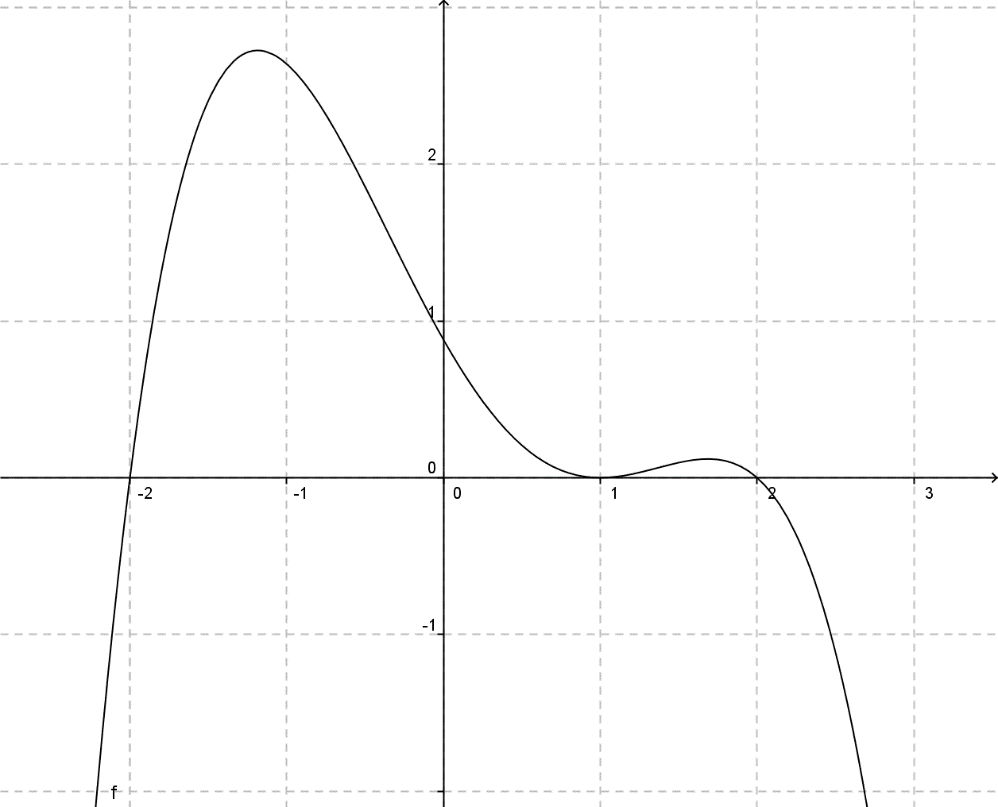
\includegraphics{210227.png}
\end{figure}

\newpage


\Aufgabe{2: Stochastik}
Gegeben ist eine Zufallsgröße $X$, die die Werte $x_i = \{-2; 0; 2; 4\}$ annimmt.\\
Dem untenstehenden Histogramm kann man die Wahrscheinlichkeitswerte $P(X = x_i)$ entnehmen



\begin{figure}[h!]
  \centering
\begin{tikzpicture}[>=latex, line cap=round, line join=round,>=triangle 45]
\begin{axis}[
  %unit vector ratio=1 10,
  axis x line=center,
  axis y line=center,
  axis line style = thick,
  xtick align=inside,
  %extra x tick style={tick style={very thick}}
  xtick={-4,-2,0,2,4},
  ytick={0,0.1,0.2,0.3,0.4},
  xtick style=thick,
  ytick style=thick,
  xticklabels={,,},
  extra x ticks={-2,0,2,4},
  bar width=1cm,
  %xticklabel style={anchor=south west},
  %minor x tick num=1,
  %minor y tick num=1,
  %minor tick num = 1,
  x=1cm,    %größe der kästchen in x-richtung
  y=10cm,    %größe der kästchen in y-richtung
  xlabel={$x$},
  ylabel={$P(X=x)$},
  ymajorgrids=true,
  xlabel style={below right},
  ylabel style={below right},
  %xmajorgrids=true,
  xmin=-4,
  xmax=5,
  ymin=0,
  ymax=0.4]

\addplot[ybar,fill=blue,fill opacity=0.2] coordinates {
        (-2,0.2)
        (0,0.3)
        (4,0.2)
    };
\end{axis}
\end{tikzpicture}
\end{figure}

%\begin{figure}[h!]
%  \centering
%  \includegraphics[width=0.5\columnwidth]{210227_barChart_p.png}
%\end{figure}

Ergänzen Sie den zu $x_i=2$ gehörenden Wahrscheinlichkeitswert im Histogramm und ermitteln Sie näherungsweise den Erwartungswert der Zufallsgröße.

\Aufgabe{3 Geometrie:}

 Gegeben sind die Punkte  $ O(0 | 0 |0)$, $ B(0 | 1 |0)$, $ P(t | 0 |t)$ und $ Q(1-2t | t |t)$ mit einem  Parameter $t \in R$

\begin{enumerate}[label={\alph*)}] 
\item Stellen Sie für $t=\frac{1}{2}$ Gleichungen für die Geraden $BP$ und $OQ$ auf.
\item Für welchen Wert von $ t$ sind die Richtungsvektoren von $BP$ und $OQ$ linear abhängig? Begründen Sie ihre Antwort.
\item Bestimmen Sie den  Wert von t, für welchen die  Geraden $BP$ und $OQ$ einen Schnittpunkt $S$ besitzen. Berechnen Sie dann die Koordinaten dieses Schnittpunktes $S$.
\end{enumerate}



\newpage
\enlargethispage{2cm}
{TEIL B} - mit Hilfsmittel


\Aufgabe{4: Analysis}
Gegeben sei die Funktion $f: x\rightarrow \frac{1}{2}x\cdot e^{-0.1x+2}$. Die Funktion hat bei $x=0$ ihre einzige Nullstelle.\\
Ihr Graph ist in der Abbildung dargestellt.\\
Die Funktion $F:x\rightarrow (-5x-50)\cdot e^{-0.1x+2}$ ist eine Stammfunktion der Funktion $f$.

\begin{figure}[H]
  \centering

    \subfloat[]{

\begin{tikzpicture}[>=latex, x=1cm, y=1cm, line cap=round, line join=round,>=triangle 45]
\begin{axis}[
  unit vector ratio=1 2,
  axis x line=center,
  axis y line=center,
  axis line style = thick,
  %extra x tick style={tick style={very thick}}
  xtick={-10,0,...,50,60},
  ytick={-10,-5,...,5,10},
  ticklabel style={fill=white},
  %extra x ticks={0},
  %xticklabel style={anchor=south west},
  %minor x tick num=1,
  %minor y tick num=1,
  %minor tick num = 1,
  %x=1cm,    %größe der kästchen in x-richtung
  %y=1cm,    %größe der kästchen in y-richtung
  xlabel={$x$},
  ylabel={$y$},
  grid=both,
  grid=major, grid style={dashed,gray!30},
  grid=minor, grid style={dashed,gray!30},
  ymajorgrids=true,
  xmajorgrids=true,
  xlabel style={below right},
  ylabel style={above left},
  xmin=-15.5,
  xmax=65.5,
  ymin=-10.5,
  ymax=14]
%\coordinate (O) at (0,0)
%\addplot [mark=none,domain=-15:15] {};
% \draw[line width=1pt,color=ccqqqq,smooth,samples=100,domain=-15:65] plot(\x,{0.5*\x *e^(-0.1*\x+2)});
%        \draw[line width=1pt,color=ccqqqq,smooth,samples=100,domain=-15:65] plot(\x,{50 *\x+2});
    \draw[line width=2pt,color=qqwuqq,smooth,samples=100,domain=-21.518627341217258:25.46534828151831] plot(\x,{5*((\x)^(2)/3-(\x)^(3)/20)});
  %\addplot[line width=1pt,color=ccqqqq, domain=-15:65]plot(\x,{0.5*\x*e^(-0.1*\x+2)});
%\draw (26.07701146189816,9.323776772024983) node[anchor=north west] {$G_f$};

\end{axis}
\end{tikzpicture}

        %\addplot[line width=1pt,color=ccqqqq ]plot(\x,{0.5*\x*e^(-0.1*\x+2)});

%\draw (26.07701146189816,9.323776772024983) node[anchor=north west] {G_f};
%\begin{scriptsize}
%\draw[color=ccqqqq] (0.06341005665314936,-6.095192074225563) node {$f$};
%\end{scriptsize}
%\end{axis}
%\end{tikzpicture}

    }

\end{figure}


\begin{enumerate}[label={\alph*)}]
\item Bestimmen Sie das Krümmungsverhalten der Funktion $f$ sowie die Lage des Wendepunkts.\\
  \item Der Graph der Funktion $f$ und die Gerade $ g: x\rightarrow0,5 x$ schließen im 1. Quadranten ein Flächenstück ein. Bestimmen Sie dessen Wert und interpretieren Sie diesen Wert geometrisch in der obigen Abbildung.
\end{enumerate}


\Aufgabe{5: Stochastik}
Beim Spielen mit einem Würfel stellt der Stefan fest, dass die Augenzahl 1 überdurchschnittlich häufig, die Augenzahl 6 dagegen relativ selten auftritt. Diese führt zu der Vermutung, dass der Würfel gezinkt ist und die Wahrscheinlichkeit eine 6 zu würfeln, nur $10$ beträgt. Gehen Sie zunächst davon aus, dass die Vermutung zutrifft.
Mit dem Würfel wird 100-mal nacheinander gewürfelt. Die Zufallsgröße X zählt die Anzahl der Sechsen.
\begin{enumerate}[label={\alph*)}]


\item Berechnen Sie die Wahrscheinlichkeit, dass in 100 Würfen genau 10 Sechsen auftreten.
\item Berechnen Sie die Wahrscheinlichkeit, dass in 100 Würfen mindestens 16 Sechsen auftreten.
\item Berechnen Sie Erwartungswert $\mu$ und Standardabweichung $\sigma$ und bestimmen Sie die Wahrscheinlichkeit, dass X um höchstens $1,5 \sigma$ von $ \mu$ abweicht.\\
Mit dem Würfel wird mehrmals nacheinander gewürfelt.
\item Ermitteln Sie, wie oft ein Spieler mindestens würfeln muss, um einer Wahrscheinlichkeit von wenigsten 95\% mindestens einmal eine 6 zu erhalten.
\item Bestimmen Sie die Wahrscheinlichkeit, dass erst im fünften Wurf zum ersten Mal eine Sechs auftritt.
\end{enumerate}


\newpage

\enlargethispage{2cm}
\Aufgabe{6: Geometrie}
Eine ägyptische Pyramide hat die Form einer geraden quadratischen Pyramide. Die Seitenlänge des Grundquadrats beträgt 160m, die Höhe der Pyramide 100m. Im Modell in einem Koordinatensystem mit Längeneinheit 1m liegt der Ursprung genau in der Mitte der quadratischen Grundfläche und die $x_1$- und $x_2$-Achse verlaufen parallel zu den Grundkanten. 

  \begin{figure}[H]
    \centering
    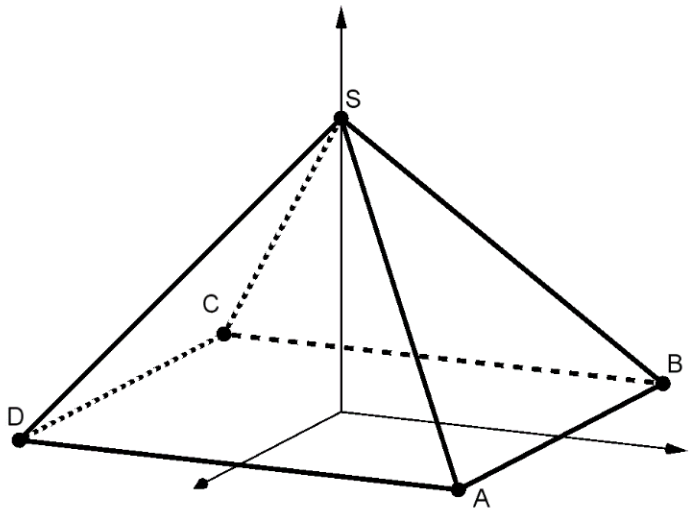
\includegraphics[width=0.5\columnwidth]{210227_pyramide.png}
    %\caption{A boat.}
    %\label{fig:boat1}
  \end{figure}




\begin{enumerate}[label={\alph*)}]
  \item Geben Sie die Koordinaten der Eckpunkte $A$,$B$ und $S$ an und bestimmen Sie die Gleichung der Ebene $E$ durch diese Punkte in Koordinatenform.\\
    {\it [mögliches Teilergebnis: $E: 5x_2 + 4x_3 = 400$]}
  \item Die Ägypter bauten die Pyramide schichtweise. Zum Transport der Steine zur jeweiligen Schicht wurde eine Rampe benötigt. Die Rampe führt enlang der Geraden\\

\[
\begin {aligned}
    r: \vec{X}= \begin{pmatrix} 0 \\
                              200 \\
                                0
                  \end{pmatrix}
           + \mu \begin{pmatrix} 0 \\
                                24 \\
                                -5
                  \end{pmatrix}
\end {aligned}
\qquad
\qquad
\raisebox{-10mm}{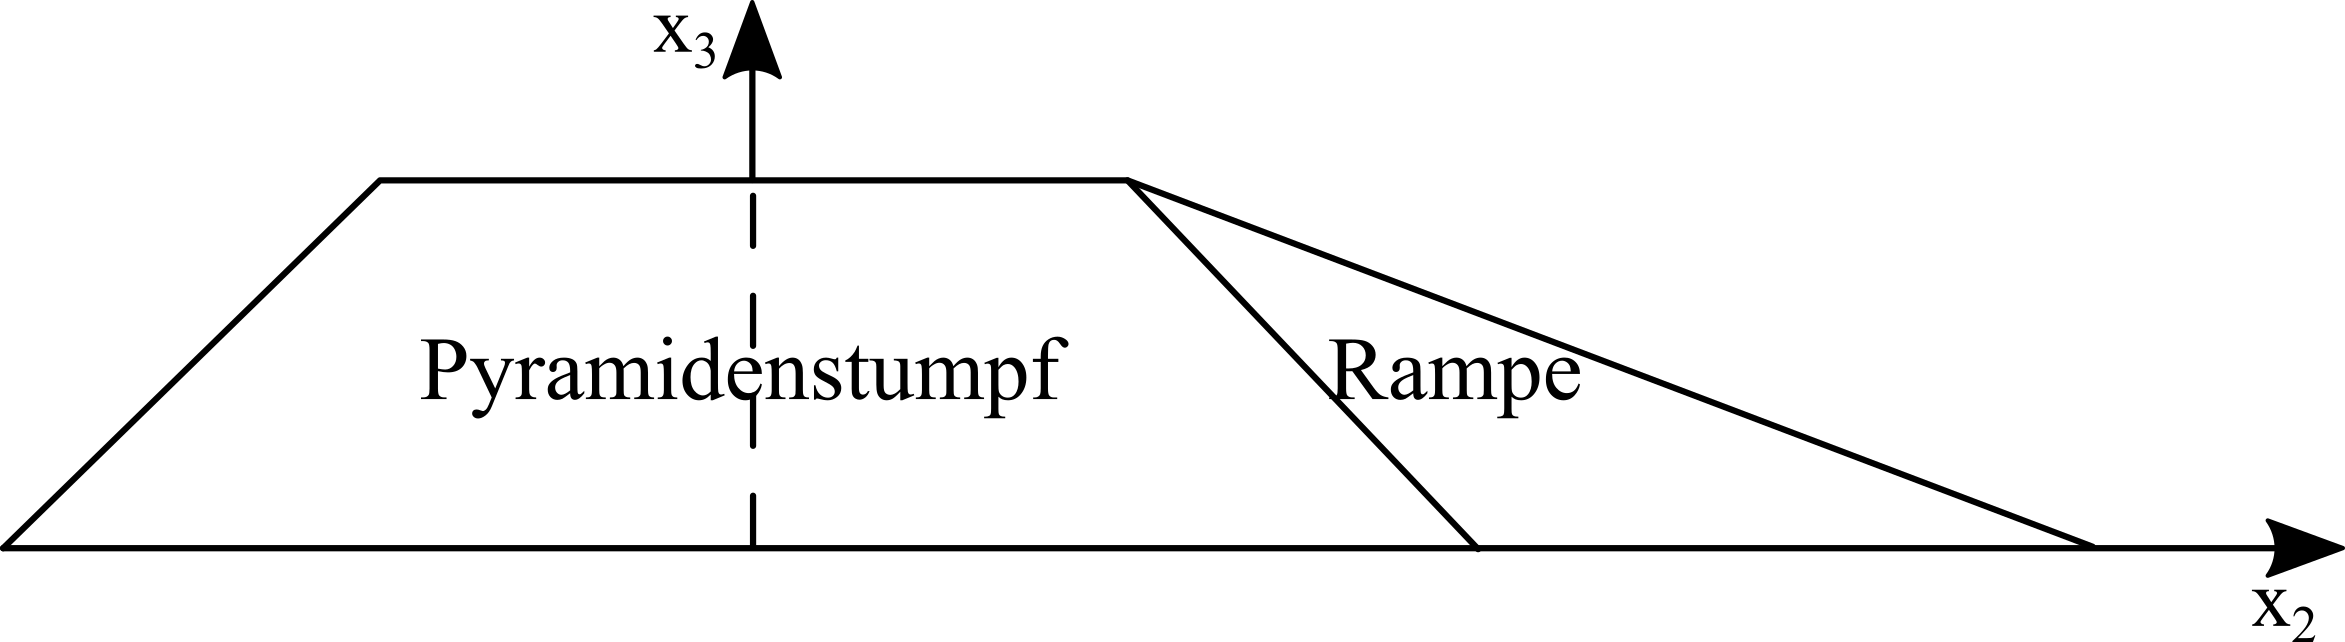
\includegraphics[keepaspectratio = true, scale = 0.5] {210227_pyramidenStumpfRampe.png}}
\]


  vom Erdboden bis an den Rand des bisher errichteten Pyramidenstumpfs und liegt in der $x_2-x_3$ Ebene.\\
    
    Berechnen Sie die Höhe des bisher gebauten Pyramidenstumpfes und die Länge der Rampe.\\

  \item  Der Punkt T$(0|60|25)$ liegt auf der Seitenfläche $ABS$. Er ist der Einstiegspunkt zu einem Schacht, der senkrecht zu dieser Seitenfläche verläuft und in 13m Höhe über der Grundfläche am Eingang der inneren Grabkammer endet. Berechnen Sie die Koordinaten dieses Endpunkts.
\end{enumerate}



\centerline{Viel Erfolg}
%\enlargethispage{2\baselineskip}

%\addtolength{\voffset}{-2cm}




%\begin{tikzpicture}
%\draw [very thin, black, step=0.5cm] (0,0) grid +(15,18);
%\end{tikzpicture}




%%%%%%%%%%%%%%%%%%%%%%%%%%%%%%%%%%%%%%%%%%%%%%%%%%%%%%
%%%%%%%%%%%%%%%%%%%%%%%%%%%%%%%%%%%%%%%%%%%%%%%%%%%%%%
\end{document}
